\documentclass[border=10pt,tikz]{standalone}
\usepackage{graphicx}
% \usepackage{tikz}

\usetikzlibrary{arrows.meta}

\definecolor{gold}{HTML}{ffd700}
\definecolor{blue}{HTML}{5700ff}
\definecolor{red}{HTML}{ff5700}

\begin{document}

\begin{tikzpicture}
\node[anchor=south west,inner sep=0] (image) at (0,0) {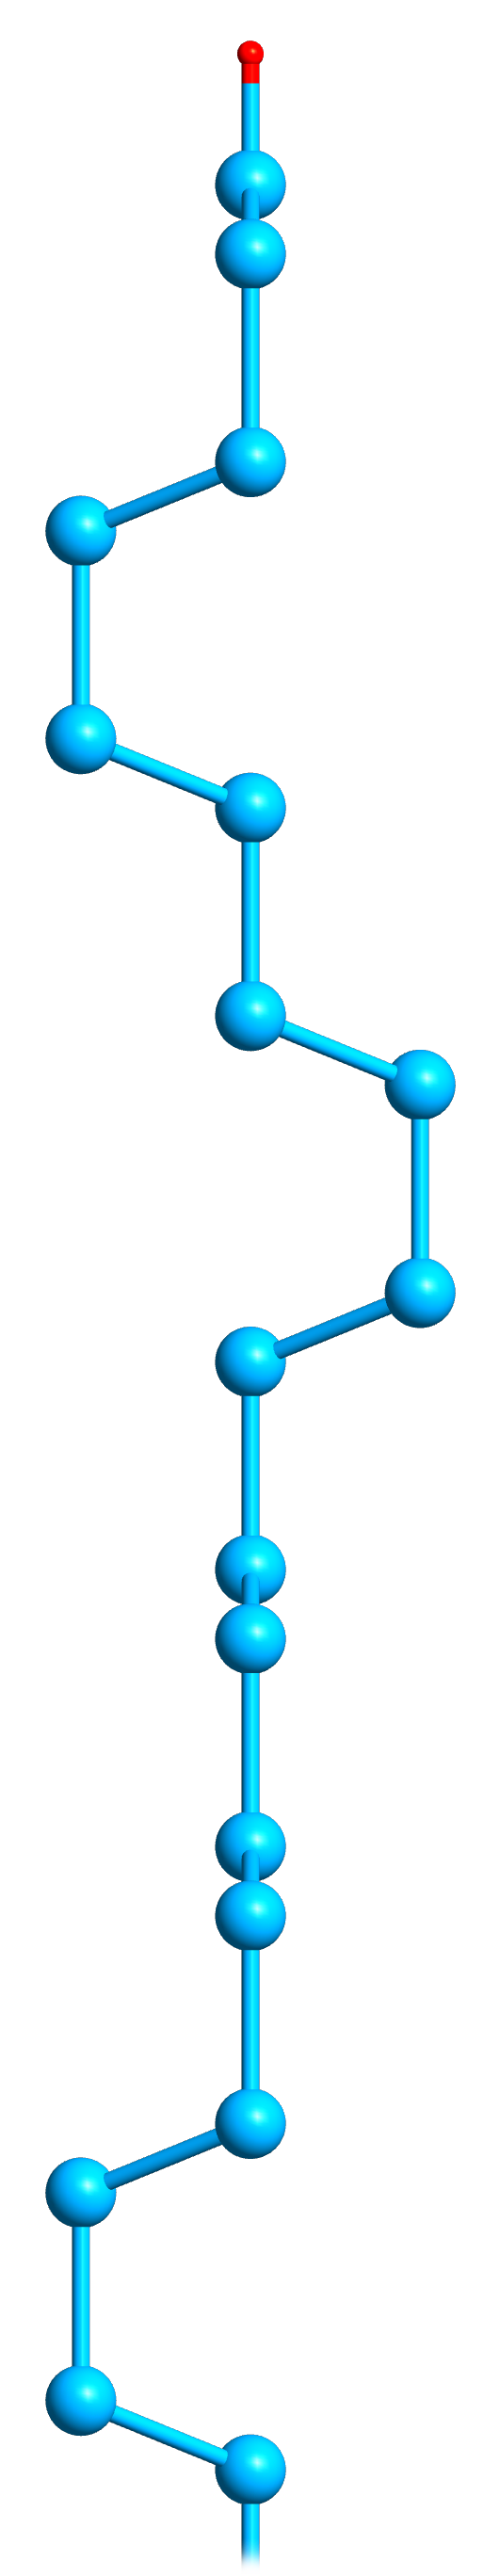
\includegraphics[scale=0.125]{../png/36layer_hs-yz.png}};

% axes
\draw [-Latex, line width=1pt] (3,12) -- ++(1,0) node [below] {{$y$}};
\draw [-Latex, line width=1pt] (3,12) -- ++(0,1) node [right] {{$z$}};
\draw [fill=white, line width=1pt] (3,12) circle (0.1) node [left,xshift=-3pt, yshift=-5pt] {{$x$}};
\fill (3,12) circle (0.03);

\begin{scope}[x={(image.south east)}, y={(image.north west)}]
    % atom names and layers
    \node [anchor=west] at (+0.55,0.98) {H$_{1}$};
    \node [anchor=west] at (+0.58,0.93) {Si$_{2}$};
    \node [anchor=west] at (+0.12,0.90) {Si$_{3}$};
    \node [anchor=west] at (+0.58,0.82) {Si$_{4}$};
    \node [anchor=west] at (-0.22,0.79) {Si$_{5}$};
    \node [anchor=west] at (-0.22,0.71) {Si$_{6}$};
    \node [anchor=west] at (+0.58,0.69) {Si$_{7}$};
    \node [anchor=west] at (+0.12,0.60) {Si$_{8}$};
    \node [anchor=west] at (+0.90,0.58) {Si$_{9}$};
    \node [anchor=west] at (+0.90,0.49) {Si$_{10}$};
    \node [anchor=west] at (+0.12,0.47) {Si$_{11}$};
    \node [anchor=west] at (+0.58,0.39) {Si$_{12}$};
    \node [anchor=west] at (+0.12,0.36) {Si$_{13}$};
    \node [anchor=west] at (+0.58,0.28) {Si$_{14}$};
    \node [anchor=west] at (+0.12,0.25) {Si$_{15}$};
    \node [anchor=west] at (+0.58,0.17) {Si$_{16}$};
    \node [anchor=west] at (-0.22,0.15) {Si$_{17}$};
    \node [anchor=west] at (-0.22,0.07) {Si$_{18}$};
    \node [anchor=west] at (+0.58,0.04) {Si$_{19}$};
\end{scope}
\end{tikzpicture}

\end{document}
